%------------------------------- CHAPTER NAME --------------------------------
\chapter{Software overview}
%------------------------------- MAIN PURPOSES -------------------------------
\section{Main purposes}
This thesis deals with the development of a software framework that could help, during preliminary and conceptual design phases, in finding a configuration which satisfies several basic requirements and, eventually, a constrained optimum. 

\bigskip
\noindent
Since the end of 80’s many software dealing with aircraft design have been produced with the aim of having some design framework to be used for teaching and professional purposes in aircraft design. However, some new software have recently followed innovative approaches, considering concepts like \gls{KBE} and \gls{MDO}, and have highlighted the necessity of an efficient graphical user interface in order to make results easily exploitable with external software.
%
The software in exam has been designed to embrace different types of analysis pertaining disciplines such as Aerodynamics, Structures, Weights and Propulsion. Furthermore, since in the conceptual and preliminary design phases a lot of different configurations have to be analyzed, the latter has been conceived to provide results in a relatively short computational time. This need often requires to rely on semi-empirical methods so that, to improve their accuracy, a comprehensive study of the methods available in literature has been firstly carried out; each method has been tested against experimental data (produced in-house or
drawn from literature) so that statistical quantities could be estimated either to find the best method currently available or to make a merger of different methods.
Whenever possible, application results have been compared with values found in literature or in-house databases.\cite{attanasio}

%-------------------------------AIRCRAFT DESIGN -------------------------------
\subsection{Aircraft design ovrewiev}
Modern aerospace design begins with the desire of mankind to achieve powered, heavier-than-air flight. Early aerospace designs were characterized not only by a great deal of trial and error but also by a not inconsiderable amount of analysis. As the technologies used in aerospace applications
have developed, the goals have become vastly more sophisticated.

\noindent
It is possible to view the first 75 years of aerospace design as a series of stages: first came the early pioneers, working at a time when many were skeptical about the benefits of flight or even if it was possible at all. Next came the phase where outstanding individuals dominated aeronautical science and design during the interwar and early postwar years. This was followed in the 1950s and 1960s by a greater emphasis on design teams and the massive expansion of the great aerospace companies that we recognize today, such as Lockheed Martin and Rolls-Royce. Following these stages, the advent of \gls{acr:CAE}, design and  manufacture in the mid-1970s transformed activities in aerospace with an increasing focus on faster design cycles, more accurate predictive capabilities and the rise of computer science. At the same time, the great drawing offices of the 1950s declined and fewer people were involved in the design of each individual component.\cite{gambardella}

\bigskip
\noindent
Recent developments in information technology have had a major impact upon the aeronautical design process. The emphasis has become one where the whole design procedure from concept to the derivation of manufacturing data is covered by an integrated information technology system. Computer aided design techniques are used to produce digital data for, for example, application to numerically controlled machining. Virtual reality concepts are employed to visualise threedimensional installation and operational aspects, at least in part replacing full-scale mockups. While these procedures are particularly relevant to the detail phases of the design process their application commences as soon as a requirement is defined and numerical data are derived from it.\cite{howe2000aircraft}

\bigskip
\noindent
The design of an aircraft is a large undertaking, requiring the team efforts of many engineers having expertise in the areas of aerodynamics, propulsion, structures, flight control, performance, and weights. As the design takes shape, specialists are called into design such components as the crew station, landing gear, interior layout, armament location, and equipment installation. The completed aircraft design is a compromise of the best efforts of many talented engineers. The different design groups they represent must work together to produce the most efficient flight vehicle. It should be clear that the design process is a very involved integration effort, requiring the pulling together and blending of many engineering disciplines.\cite{nicolai2010fundamentals}
%
\begin{figure}[!t]
\centering
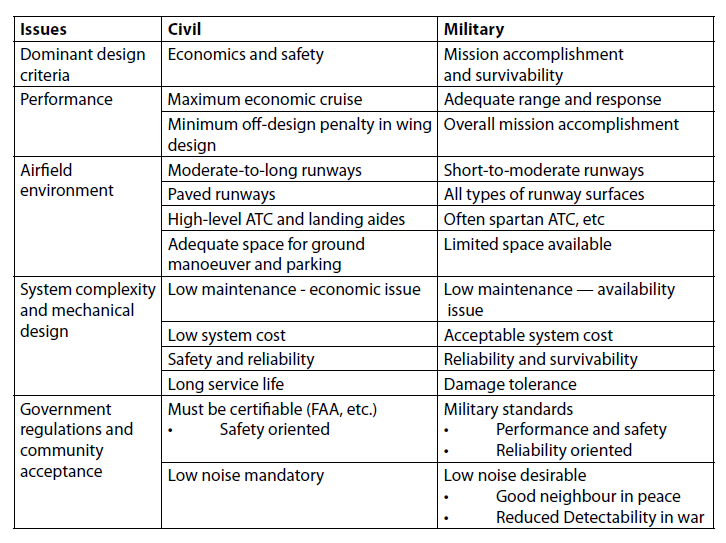
\includegraphics[keepaspectratio, width=0.8\textwidth]{DesignObjectives}
\caption{Transport aircraft design objectives and constraints. Source: \gls{acr:AIAA} Paper No 77-1795}
\label{fig:DesignObjectives}
\end{figure}

\bigskip
\noindent
A comprehensive and concise description of the general design objective of a transport aircraft can be found in \cite{obert2009aerodynamic}; here this objective is described as the transport of a payload over a distance between airports against minimum costs (for example at an optimum speed).
The driving parameters to accomplish this goal are the followings.
%
\begin{itemize}
\item Engine characteristics
\item Aerodynamic efficiency, $C_{L\text{max}}$, buffet boundary
\item Weight
\end{itemize}
%
It should be emphasised that estimating the weight and aerodynamic characteristics with sufficient accuracy at an early stage of the design is really an art, but an important one and a crucial one; in fact, it determines the initial quality of the design.
%
The airworthiness requirements then require the aircraft to be safe, for example its flight handling characteristics (stability and control) must be satisfactory. The aircraft should also be reliable, which implies that:
%
\begin{itemize}
\item Systems (such as navigation equipment) must be adequate
\item Systems hall be reliable and sufficiently redundant
\end{itemize}
%
In civil air transport, designing a family of aircraft has become a standard procedure. Two approaches can be recognised.
%
\begin{itemize}
\item In the first approach, several versions of the aircraft are developed more or less simultaneously from the start of a programme. These different versions can have different take-off weights, fuselage lenghts, etc.
\item In the second approach, growth versions of the aircraft are developed (long) after the first development round has been completed. These growth versions usually have considerable modifications and associated costs
\end{itemize}
%
Figure \ref{fig:DesignObjectives} summarizes the main design objectives to be followed in both a civil or a military aircraft project.

\bigskip
\noindent
Prior to designing any new aircraft, it is essential to see what the competition is offering. If the designed aircraft is not decidedly better than what exists in the market, it would be foolish to “bet your company” on developing a new design. The market survey should rigorously examine three or four existing aircraft for
which information is available and which most closely satisfy the assigned mission.\cite{sforza2014commercial}

\bigskip
\noindent
After the market survey phase is complete, the aircraft design process can start. Generally speaking it involves several distinct phases which can be resumed as follows.
%
\begin{enumerate}
\item \textbf{Requirements phase}
\item \textbf{Conceptual design phase}, which encompasses sizing of the most promising overall aircraft concept and proof of its feasibility. Having a typical duration between 4 to 6 months for a business aircraft and 9 to 12 months for a mid-size airliner, conceptual design is characterized by cyclic design improvements and complexity increasing in time
\item \textbf{Preliminary design phase}, which aims at specifying the design concept at the main component level, sometimes including subsystem trades. Preliminary design typically lasts between 12 and 16 months
\item \textbf{Detail design phase} which begins when a management decision is taken to continue and give the project go-ahead. This development phase is entered soon after the aircraft is committed to production and lasts between two and three years. The decision to freeze the configuration is taken early in the detail design phase when changes in the product definition are no longer appropriate.
\item \textbf{Proof of concept aircraft construction and testing phase}
\end{enumerate}
%
\begin{figure}[!t]
\centering
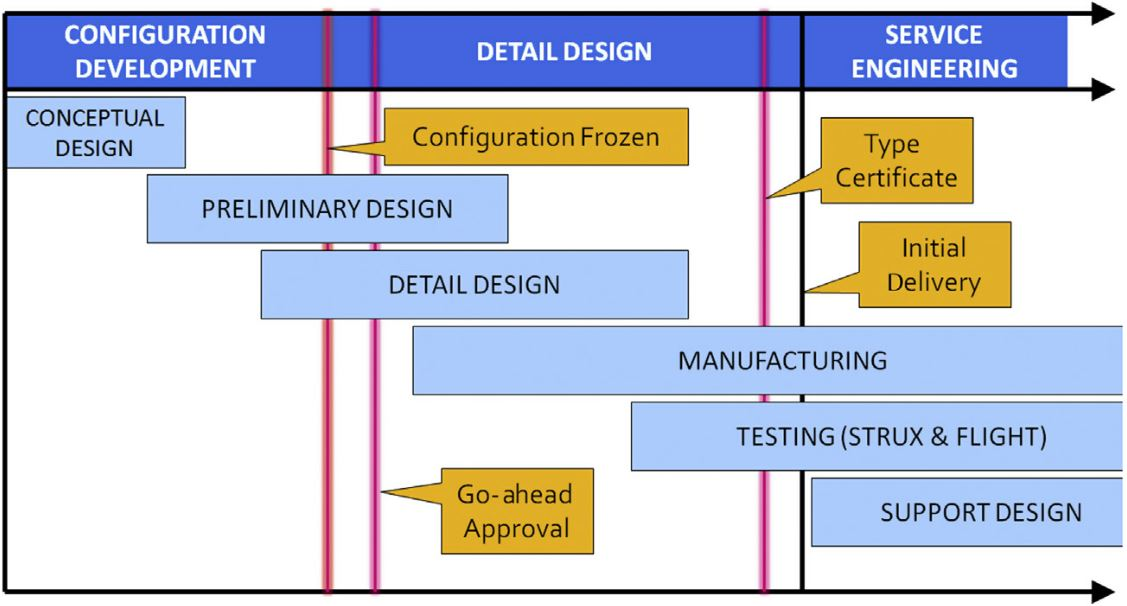
\includegraphics[scale=0.45]{Process_Design_Torenbeek}
\caption{Aircraft design process for Torenbeek (\num{1986})}
\end{figure}
%
%-------------------------------JAVA LANGUAGE---------------------------------
\subsection{Java: motivation and main features}
The choice of Java as the programming language was driven by several considerations, as explained in \cite{adoptunina}. These include the following:
%
\begin{itemize}
\item The language should be widely supported; this to avoid the case of many valid aircraft design applications and libraries that became obsolete due to the aging of the programming language used to build them
\item The language should promote the use of open source libraries, especially for I/O tasks and for complex mathematical operations
\item The language and the companion \gls{IDE} should provide a widely supported\gls{acr:GUI} framework and a \gls{acr:GUI} visual builder
\item The language should support and promote modularity
\end{itemize}
%
The Java programming language meets all these requirements; moreover it is backed by Oracle and by a huge community of developers so it is continuously updated. Also, advanced and free \gls{IDE}s (such as Eclipse or Netbeans) allow programmers to streamline and simplify the development process; in particular, the Eclipse \gls{IDE} has been chosen to develop software.
%
Being Java a pure object oriented programming language, it greatly encourages and simplifies modularization. Each module (package) can be programmed quite independently so that it is relatively easy to divide the work among several programmers. This is essential since the amount of classes and calculations needed to abstract, manage and analyze the entire aircraft is very large (presently the whole project counts more than 56000 lines of code). For such a reason the establishment of common practices and the adherence to fundamental principle of software development (\emph{Don’t Repeat Yourself}, \emph{Separation of Concerns}, \emph{Agile software development}) are equally important.

\bigskip
\noindent
According to the TIOBE index, in terms of popularity, during the last year the Java language has proven to be the most used among the developers community as shown in the following figure. 
%
\begin{figure}[H]
\centering
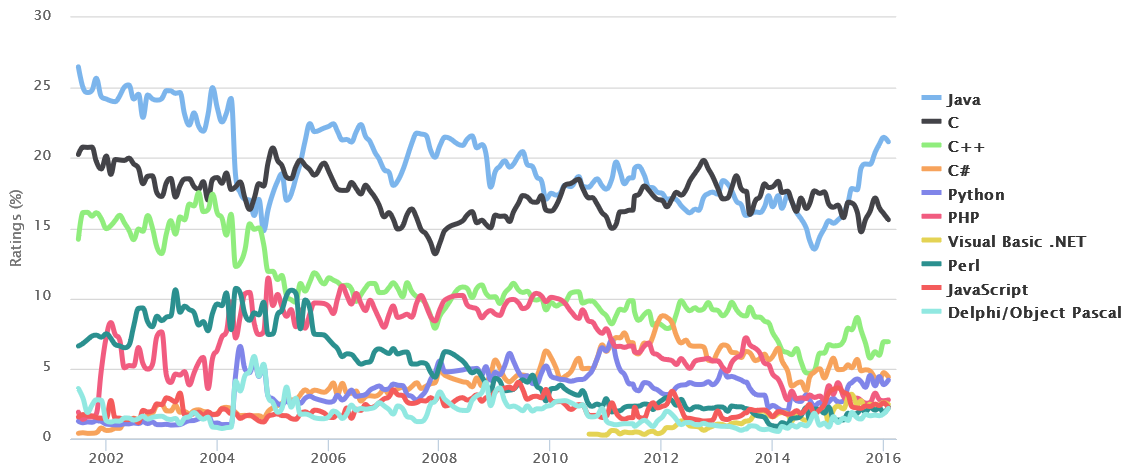
\includegraphics[scale=0.7]{LanguageTrend}
\caption{TIOBE Programming Community Index (www.tiobe.com)}
\end{figure}
%
%--------------------------- INPUT FILE STRUCTURE ---------------------------
\section{Input file structure}

%------------------------------- CORE PACKAGE ---------------------------------
\section{\gls{JPAD} Library}

%----------------------------- DEFAULT AIRCRAFT ------------------------------
\section{Aircraft model creation} \label{par:DefaultAircraft}
In \gls{JPAD} it is possible to read an .xml file as input or generate an object whose data are written in the code. Both in the first and in the second case all needed variables are initialized with data relating the choosen aircraft. The difference between these two methods is that using an .xml file, user can define its own aircraft having a clear view about the needed data useful for the analysis. Contrariwise in order to perform test of program functionality, to use a default aircraft is the most simple way to generate a work object.

\bigskip
\noindent
Actually it is possible to define two different aircraft in order to test the functionality of the application: ATR-72 and B747-100B.
%

\bigskip
\noindent
The ATR-72, made by the French-Italian aircraft manufacturer ATR, is a stretched variant of the original ATR-42 that entered in service in 1989; it’s powered by two turboprop engine and it’s used typically as a regional airliner. The main purpose of its design was to increase the seating capacity throughout the stretching of the fuselage by 4.5m, an increased wingspan, more powerful engines and an increased fuel capacity by approximately 10$\%$.

\bigskip
\noindent
The Boeing 747 is a wide-body commercial jet airliner and cargo aircraft, often referred to by its original nickname, Jumbo Jet, or Queen of the Skies. Its distinctive hump upper deck along the forward part of the aircraft makes it among the world's most recognizable aircraft, and it was the first wide-body produced. Manufactured by Boeing's Commercial Airplane unit in the United States, the original version of the 747 had two and a half times greater capacity than the Boeing 707, one of the common large commercial aircraft of the 1960s. The four-engine 747 uses a double deck configuration for part of its length and it’s available in passenger and other versions. Boeing designed the 747's hump-like upper deck to serve as a first class lounge or extra seating, and to allow the aircraft to be easily converted to a cargo carrier by removing seats and installing a front cargo door. The 747-100B model was developed from the 747-100SR, using its stronger airframe and landing gear design; the type had an increased fuel capacity of $\SI{182000}{\liter}$, allowing for a 5000 nautical mile range with a typical 452 passengers payload, and an increased maximum take-off weight of $\SI{340000}{\kilogram}$ was offered; unlike the original 747-100, the 747-100B was offered with Pratt \& Whitney JT9D-7A, General Electric CF6-50, or Rolls-Royce RB211-524 turbofan engines.
%
\begin{figure}[H]
\centering
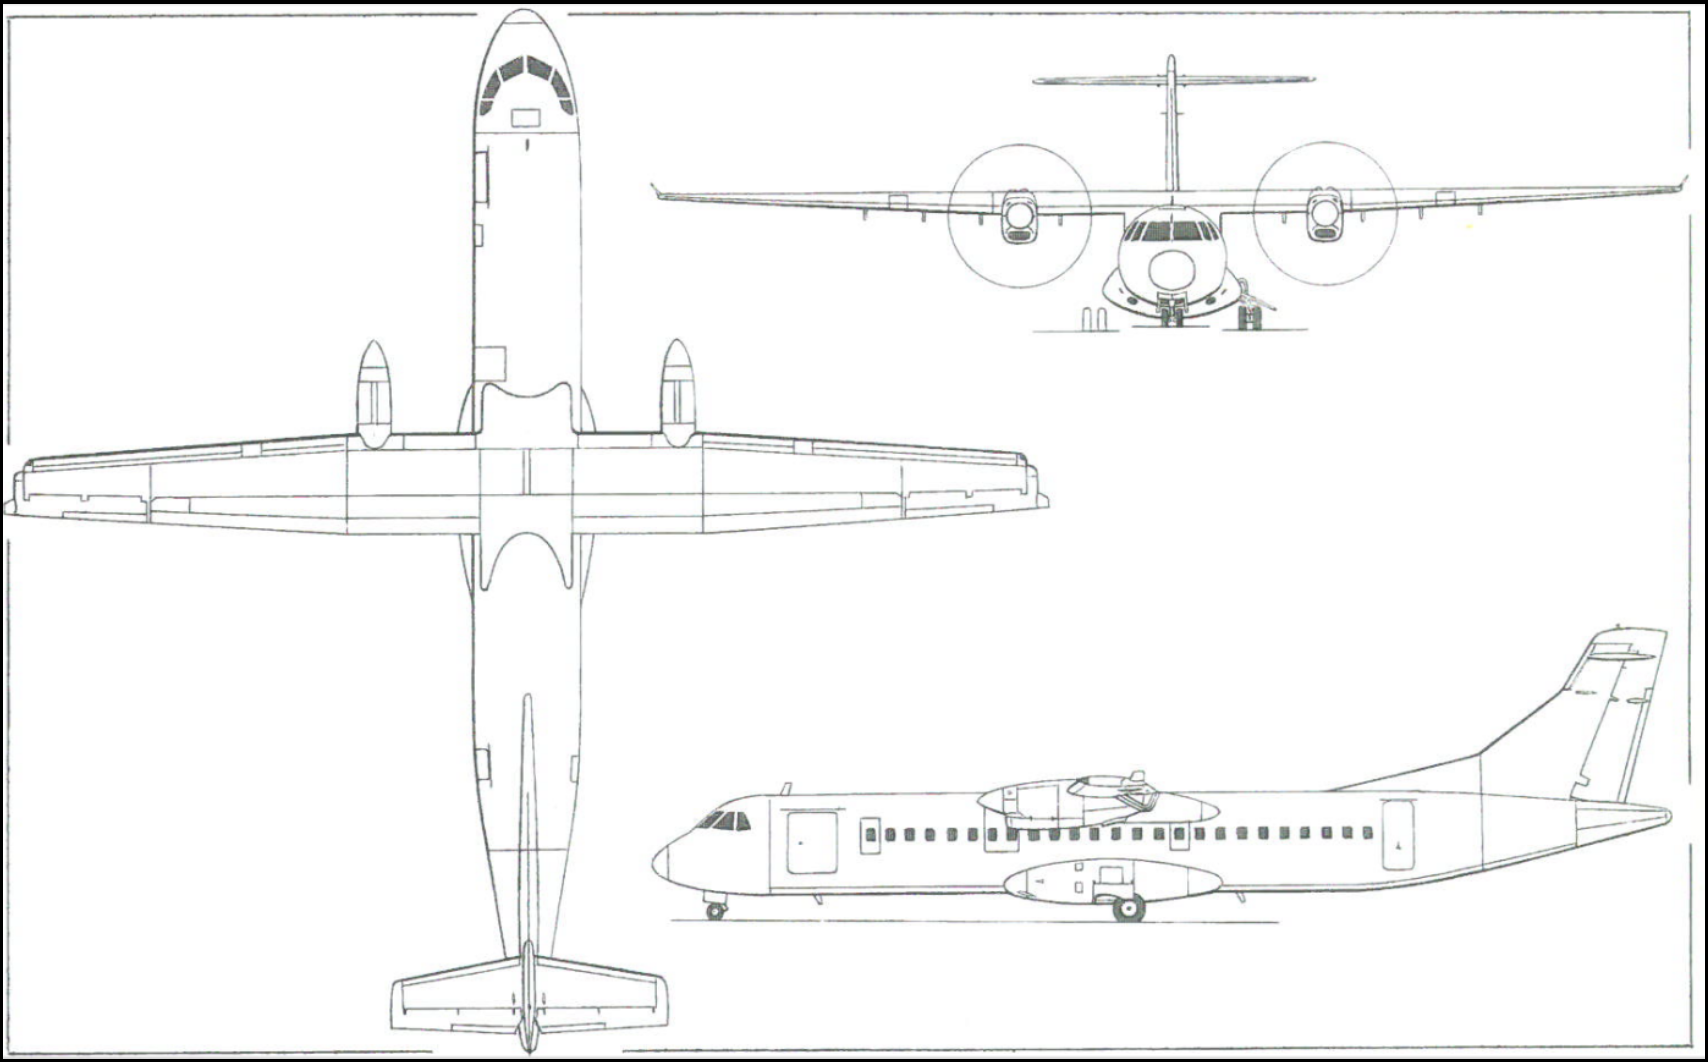
\includegraphics[keepaspectratio, width=0.8\textwidth]{ATR-72}
\caption{ATR-72 views – Jane's All the World's Aircraft 2004-2005}
\label{fig:Figure6}
\end{figure}
%
\begin{table}[h]
\makebox[\linewidth]{
\begin{tabular}{p{4cm}p{7.5cm}p{2cm}}
\toprule
\textbf{Variables} & \textbf{Description} & \textbf{Values} \\
\midrule
\lstinline[language=Java]!altitude! & Cruise altitude & $\SI{6000}{\meter}$ \\[0.2cm]
\lstinline[language=Java]!machCurrent! & The user chosen Mach number & 0,43 \\[0.2cm]
\lstinline[language=Java]!surface! & Wing surface & $\SI{61}{\meter\squared}$ \\[0.2cm]
\lstinline[language=Java]!taperRatioEquivalent! & Taper ratio of the equivalent wing & 0,545   \\[0.2cm]
\lstinline[language=Java]!maxTakeOffMass! & maximum take-off mass & $\SI{23063.5789}{\kilogram}$         \\[0.2cm]
\lstinline[language=Java]!operatingEmptyMass!	& operating empty mass & $\SI{12935.5789}{\kilogram}$ \\[0.2cm]
\lstinline[language=Java]!maxFuelMass! & maximum fuel mass & $\SI{5000.0}{\kilogram}$ \\[0.2cm]
\lstinline[language=Java]!nPassMax! & maximum number of passengers & 72 \\[0.2cm]
\lstinline[language=Java]!sweepLEEquivalent! & Equivalent wing leading edge sweep angle & $\SI{3.1415}{\degree}$ \\[0.2cm]
\lstinline[language=Java]!oswald! & Wing oswald factor & 0,7585 \\[0.2cm]
\lstinline[language=Java]!byPassRatio! & Engine bypass ratio & 0,0 \\[0.2cm]
\lstinline[language=Java]!eta! & propeller efficiency & 0,85 \\[0.2cm]
\lstinline[language=Java]!tcMax! & Mean maximum thickness of the wing & 0,1675 \\[0.2cm]
\lstinline[language=Java]!cl! & The cruise lift coefficient & 0,45 \\[0.2cm]
\lstinline[language=Java]!ar! & Wing aspect ratio & 12 \\[0.2cm]
\lstinline[language=Java]!cd0! & Wing parasite drag coefficient & 0,0317 \\[0.2cm]
\bottomrule
\end{tabular}
}
\caption{ATR-72 input data}
\label{table:Table4}
\end{table}
%
\begin{figure}[H]
\centering
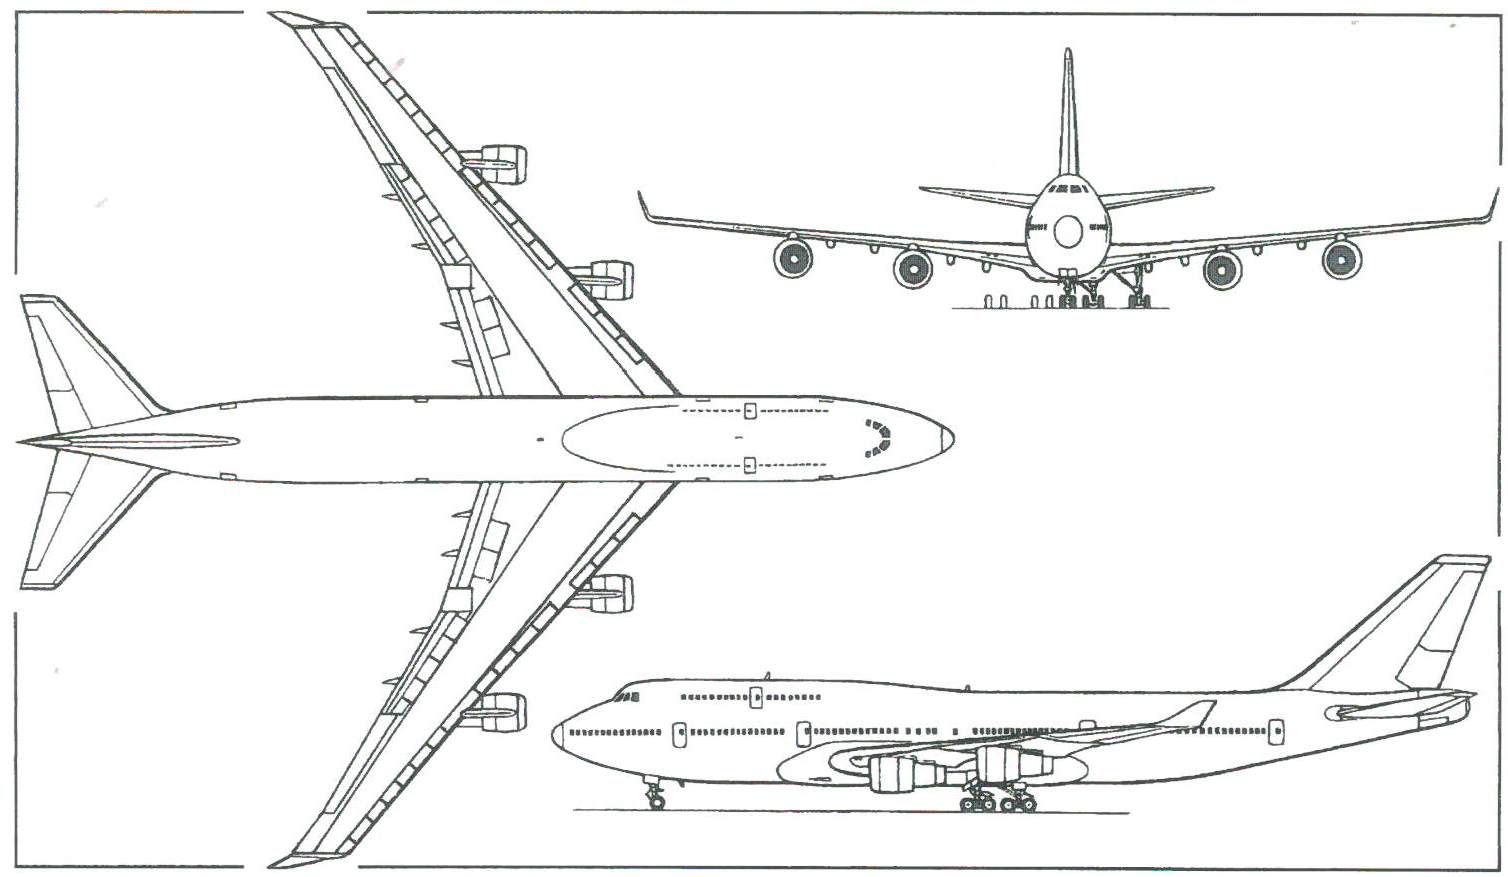
\includegraphics[keepaspectratio, width=0.85\textwidth]{B747-100B}
\caption{B747-100B views – Jane's All the World's Aircraft 2004-2005}
\label{fig:Figure7}
\end{figure}
%
\begin{table}[H]
\makebox[\linewidth]{
\begin{tabular}{p{4cm}p{7.5cm}p{2cm}}
\toprule
\textbf{Variables} & \textbf{Description} & \textbf{Values} \\
\midrule
\lstinline[language=Java]!altitude! & Cruise altitude & $\SI{11000}{\meter}$ \\[0.2cm]
\lstinline[language=Java]!machCurrent! & The user chosen Mach number & 0,83 \\[0.2cm]
\lstinline[language=Java]!surface! & Wing surface & $\SI{511}{\meter\squared}$ \\[0.2cm]
\lstinline[language=Java]!taperRatioEquivalent! & Taper ratio of the equivalent wing & 0,284   \\[0.2cm]
\lstinline[language=Java]!maxTakeOffMass! & maximum take-off mass & $\SI{354991.5060}{\kilogram}$         \\[0.2cm]
\lstinline[language=Java]!operatingEmptyMass!	& operating empty mass & $\SI{153131.9860}{\kilogram}$ \\[0.2cm]
\lstinline[language=Java]!maxFuelMass! & maximum fuel mass & $\SI{147409.52}{\kilogram}$ \\[0.2cm]
\lstinline[language=Java]!nPassMax! & maximum number of passengers & 550 \\[0.2cm]
\lstinline[language=Java]!sweepLEEquivalent! & Equivalent wing leading edge sweep angle & $\SI{38.4288}{\degree}$ \\[0.2cm]
\lstinline[language=Java]!oswald! & Wing oswald factor & 0,6277 \\[0.2cm]
\lstinline[language=Java]!byPassRatio! & Engine bypass ratio & 5,0 \\[0.2cm]
\lstinline[language=Java]!eta! & propeller efficiency & 0,0 \\[0.2cm]
\lstinline[language=Java]!tcMax! & Mean maximum thickness of the wing & 0,1292 \\[0.2cm]
\lstinline[language=Java]!cl! & The cruise lift coefficient & 0,45 \\[0.2cm]
\lstinline[language=Java]!ar! & Wing aspect ratio & 6,9 \\[0.2cm]
\lstinline[language=Java]!cd0! & Wing parasite drag coefficient & 0,0182 \\[0.2cm]
\bottomrule
\end{tabular}
}
\caption{B747-100B input data}
\label{table:Table5}
\end{table}

\bigskip
\noindent
In order to define a default aircraft in a test class, and use it to check the functionalities of the application, it is necessary to follow some steps. First of all it’s necessary to set up all default folders in order to make them achievable from any location inside the library; this is done with the static method \lstinline[language=Java]!initWorkingDirectoryTree! of the \lstinline[language=Java]!MyConfiguration! class located in \lstinline[language=Java]!JPADConfigs! package. In this way, every time the user wants to point at a specific folder, like the input or output directory, it’s necessary only to call the \gls{Static} \lstinline[language=Java]!getDir!, also from \lstinline[language=Java]!MyConfiguration! class, which reads the~folder name, from a dedicated \gls{Enum}, and associate it with the related directory from a \gls{Map} named \lstinline[language=Java]!mapPaths!.

\bigskip
\noindent
The second step is the creation of an \lstinline[language=Java]!Aircraft! object choosing between the ones grouped into a dedicated \gls{Enum}, named \lstinline[language=Java]!AircraftEnum!. This can be done using the method \lstinline[language=Java]!createDefaultAircraft! from \lstinline[language=Java]!Aircraft! class. This method defines a new \lstinline[language=Java]!Aircraft! object and invokes another method which creates all its components using default data. More in detail, inside the method \lstinline[language=Java]!createDefaultAircraft! there is a calling to the constructor of the \lstinline[language=Java]!Aircraft! class which initializes the objects of the classes that perform calculations. At this point all the components of the aircraft are created and ready to be used.

\bigskip
\noindent
Afterwards it is necessary to set the operating conditions, such as the number of Mach of analysis or the altitude, by creating an object of the class \lstinline[language=Java]!OperatingConditions!. Each default aircraft has a set of default conditions but the user could easly change them by using the \emph{setters} methods of which the \lstinline[language=Java]!OperatingConditions! class is supplied.

\bigskip
\noindent
In order to manage all the aircraft related analysis it is necessary to define an object of the class \lstinline[language=Java]!ACAnalysisManager!. Similarly to the aircraft, exists an analysis manager also for the wing that is an object of the \lstinline[language=Java]!LSAerodynamicManager! class; this results to be necessary since the aerodynamic analysis of the wing are not managed by the \lstinline[language=Java]!ACAnalysisManager! in order to allow the analysis also of an isolated wing.

\bigskip
\noindent
The next step is to define and assign the needed databases. In order to read these databases, and obtain their useful data, it is necessary to define an object
of the database reading class (see appendix \ref{par:Appendix2}) and associate it with the object of the analysis. Reading these data correctly is a crucial step; in fact, \gls{JPAD} allows to work with an \lstinline[language=Java]!Aircraft! object or only with an isolated \lstinline[language=Java]!LiftingSurface! object. The aircraft is usually composed of a fuselage, lifting surfaces, nacelle and power plant; furthermore, the aircraft and the wing are associated with different classes of calculation like \lstinline[language=Java]!ACAnalysisManager! or \lstinline[language=Java]!LSAerodynamicManager!. Since it is necessary that these databases are also visible from these classes, as well as the fact that both in aircraft and in wing there is a lifting surface object, databases relative to aerodynamic analysis are associated to \lstinline[language=Java]!LSAerodynamicManager!. 
%
In order to assign correctly this aerodynamic database and associate it to all analysis managers is necessary to practise the following order.
\begin{enumerate}
\item Define an \lstinline[language=Java]!Aircraft! Object. This command associates to the \lstinline[language=Java]!Aircraft! class an object that defines the aerodynamic. From the wing it is possible to obtain \lstinline[language=Java]!theWing!, that is a \lstinline[language=Java]!LiftingSurface! object
\item Define an \lstinline[language=Java]!ACAnalysisManager! object. All the aircraft computations are managed by this class
\item Define an \lstinline[language=Java]!LSAerodynamicManager! object. All the lifting surfaces computations are managed by this class
\item Associate database to \lstinline[language=Java]!LSAerodynamicManager!
\item Eventually do analysis. It's important to highlight that, in order to perform only an aerodynamic analysis, the user has to define manually the position of the center of gravity.
\end{enumerate} 
%
The purpose of this structure is to have only a way to assign the aerodynamic databases to an aircraft. Inasmuch as the wing is always present, the chosen strategy is to assign the database to the aerodynamic manager of the wing; moreover, in order make the database usable also by the aircraft, it is assigned at the aerodynamic manager of the aircraft by calling the method \lstinline[language=Java]!doAnalysis!. For the same reason, if the user has to get the database from the wing, the \lstinline[language=Java]!LSAerodynamicManager! object created previously has to be set as the aerodynamic analysis of the wing object. In this way it's possible to call the database using equally the following codes:
%
\begin{itemize}
\item \lstinline[language=Java]!theWingObject.getAerodynamics.get_Database!
\item \lstinline[language=Java]!theAircraftObject.get_theAerodynamic.get_Database!
\item \lstinline[language=Java]!theLSManagerObject.get_Database!
\item \lstinline[language=Java]!theACManagerObject.get_Database!
\end{itemize}
%
Although is the most important, the aerodynamic database is not the only one to be considered. To perform the high-ligt devices effects analysis (see chapter \ref{chap:HighLift}), as well as to carry out the integration of the equation of motion durign the take-off run (see chapter \ref{chap:TakeOff}), also an high-lift devices database has to be read. Since the latter is strictly related to the wing, it has to be assigned to \lstinline[language=Java]!LSAerodynamicManager! as well.

\bigskip
\noindent
The following listing shows a summary of the steps described previously in order to help a potential user to easly implement a test class inside \gls{JPAD}.

\bigskip
\begin{lstlisting}[caption={Generation of default aircraft}, captionpos=b, tabsize=2]
public static void main(String[] args) {
	// --------------------------------------------------------------
	// Define directory
	MyConfiguration.initWorkingDirectoryTree();
	// --------------------------------------------------------------
	// Generate default Aircraft
	Aircraft aircraft = Aircraft.createDefaultAircraft("B747-100B");
	LiftingSurface theWing = aircraft.get_wing();
	// --------------------------------------------------------------
	// Default operating conditions
	OperatingConditions theConditions = new OperatingConditions();		
	// --------------------------------------------------------------
	// Define an ACAnalysisManager Object
	ACAnalysisManager theAnalysis = new ACAnalysisManager(theConditions);
	theAnalysis.updateGeometry(aircraft); // required to populate aircaft derived data
	// --------------------------------------------------------------
	// Define an LSAerodynamicsManager Object
	LSAerodynamicsManager theLSAnalysis = new LSAerodynamicsManager ( 
			theConditions,
			theWing,
			aircraft
			);
	// --------------------------------------------------------------
	// Setup database(s)		
	theLSAnalysis.setDatabaseReaders(
			new Pair(DatabaseReaderEnum.AERODYNAMIC,
                          "Aerodynamic_Database_Ultimate.h5"),
			new Pair(DatabaseReaderEnum.HIGHLIFT,  
                          "HighLiftDatabase.h5")
			);
	// --------------------------------------------------------------
	// Do analysis
	theAnalysis.doAnalysis(aircraft, 
			AnalysisTypeEnum.AERODYNAMIC);
}
\end{lstlisting}
%
In conclusion the following pages shows two flowcharts useful to better understand what has been described in this paragraph.
%
\begin{figure}[H]
  \begin{adjustbox}{addcode={\begin{minipage}{\width}}{\caption{Flowchart of the creation of default Aircraft}
     \end{minipage}},rotate=90,center}
      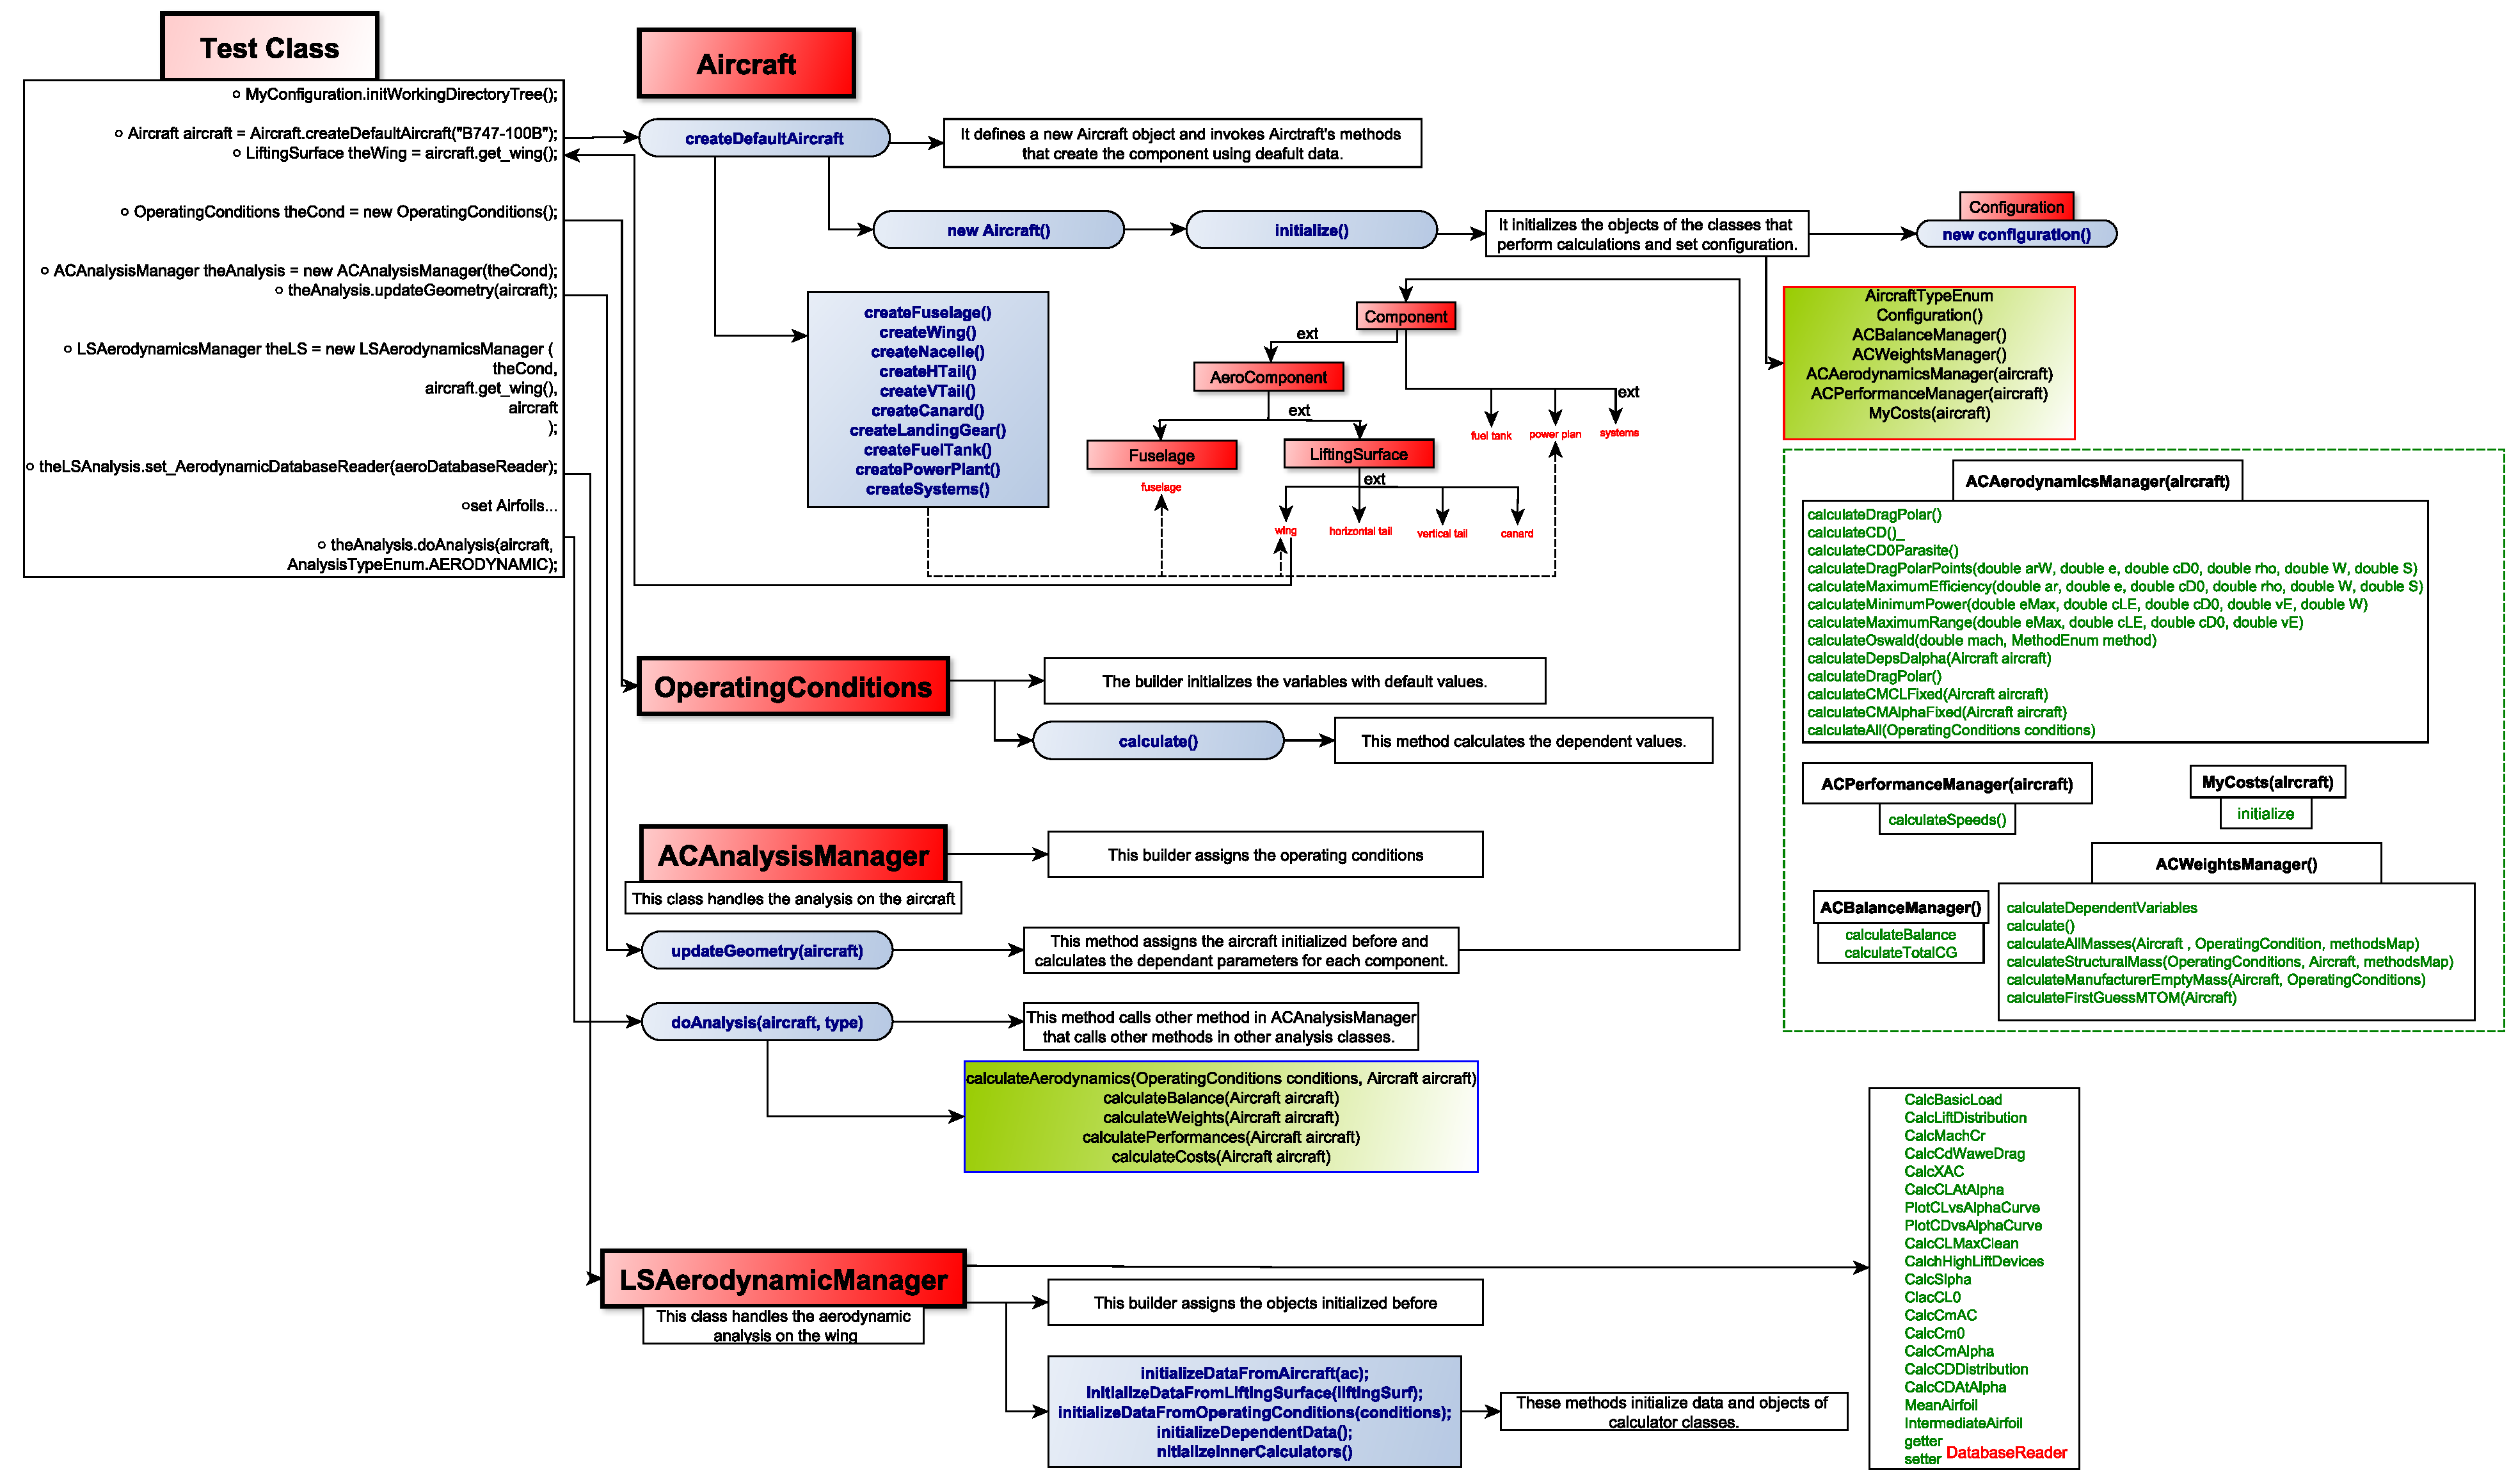
\includegraphics[scale=.38]{HowToCreateADefaultAircraftInJPAD3}
  \end{adjustbox}
\end{figure}
%
\begin{figure}[H]
  \begin{adjustbox}{addcode={\begin{minipage}{\width}}{\caption{Flowchart of database assignment}
     \end{minipage}},rotate=90,center}
      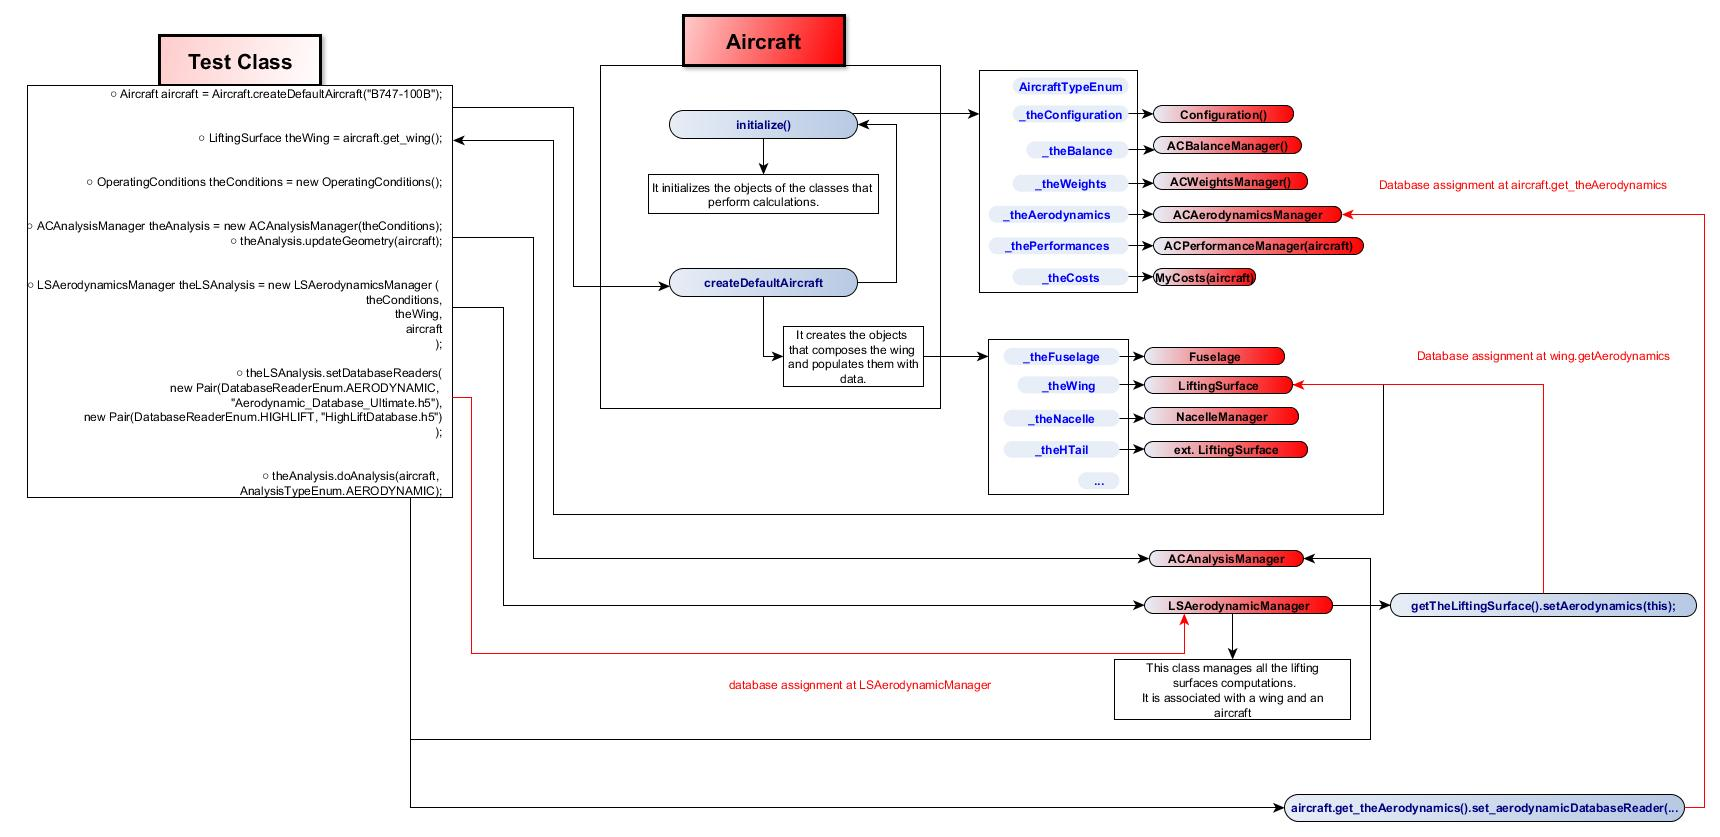
\includegraphics[scale=.42]{HowToAssignDatabase}
  \end{adjustbox}
\end{figure}
%
%---------------------------------------GUI ----------------------------------------
\section{The \gls{acr:GUI}}
An extensive work has been done to set up an effective \gls{acr:GUI} to reduce the time the user has to spend to obtain relevant results. It should be noted that this \gls{acr:GUI} is only a prototype, although fully functional, of a possible future interface still in development.

\bigskip
\noindent
The Java programming language greatly helped to build the \gls{acr:GUI}: several open source libraries (SWT, JFace) allowed to build a functional yet pleasant \gls{acr:GUI} which allows the user to easily change the aircraft parameters, to view a 3D model of the defined geometry, to launch a new analysis and view the corresponding results. The current \gls{acr:GUI} appearance is shown in figure~\ref{fig:guiStart}. 
%
\begin{figure}[h]
	\centering
	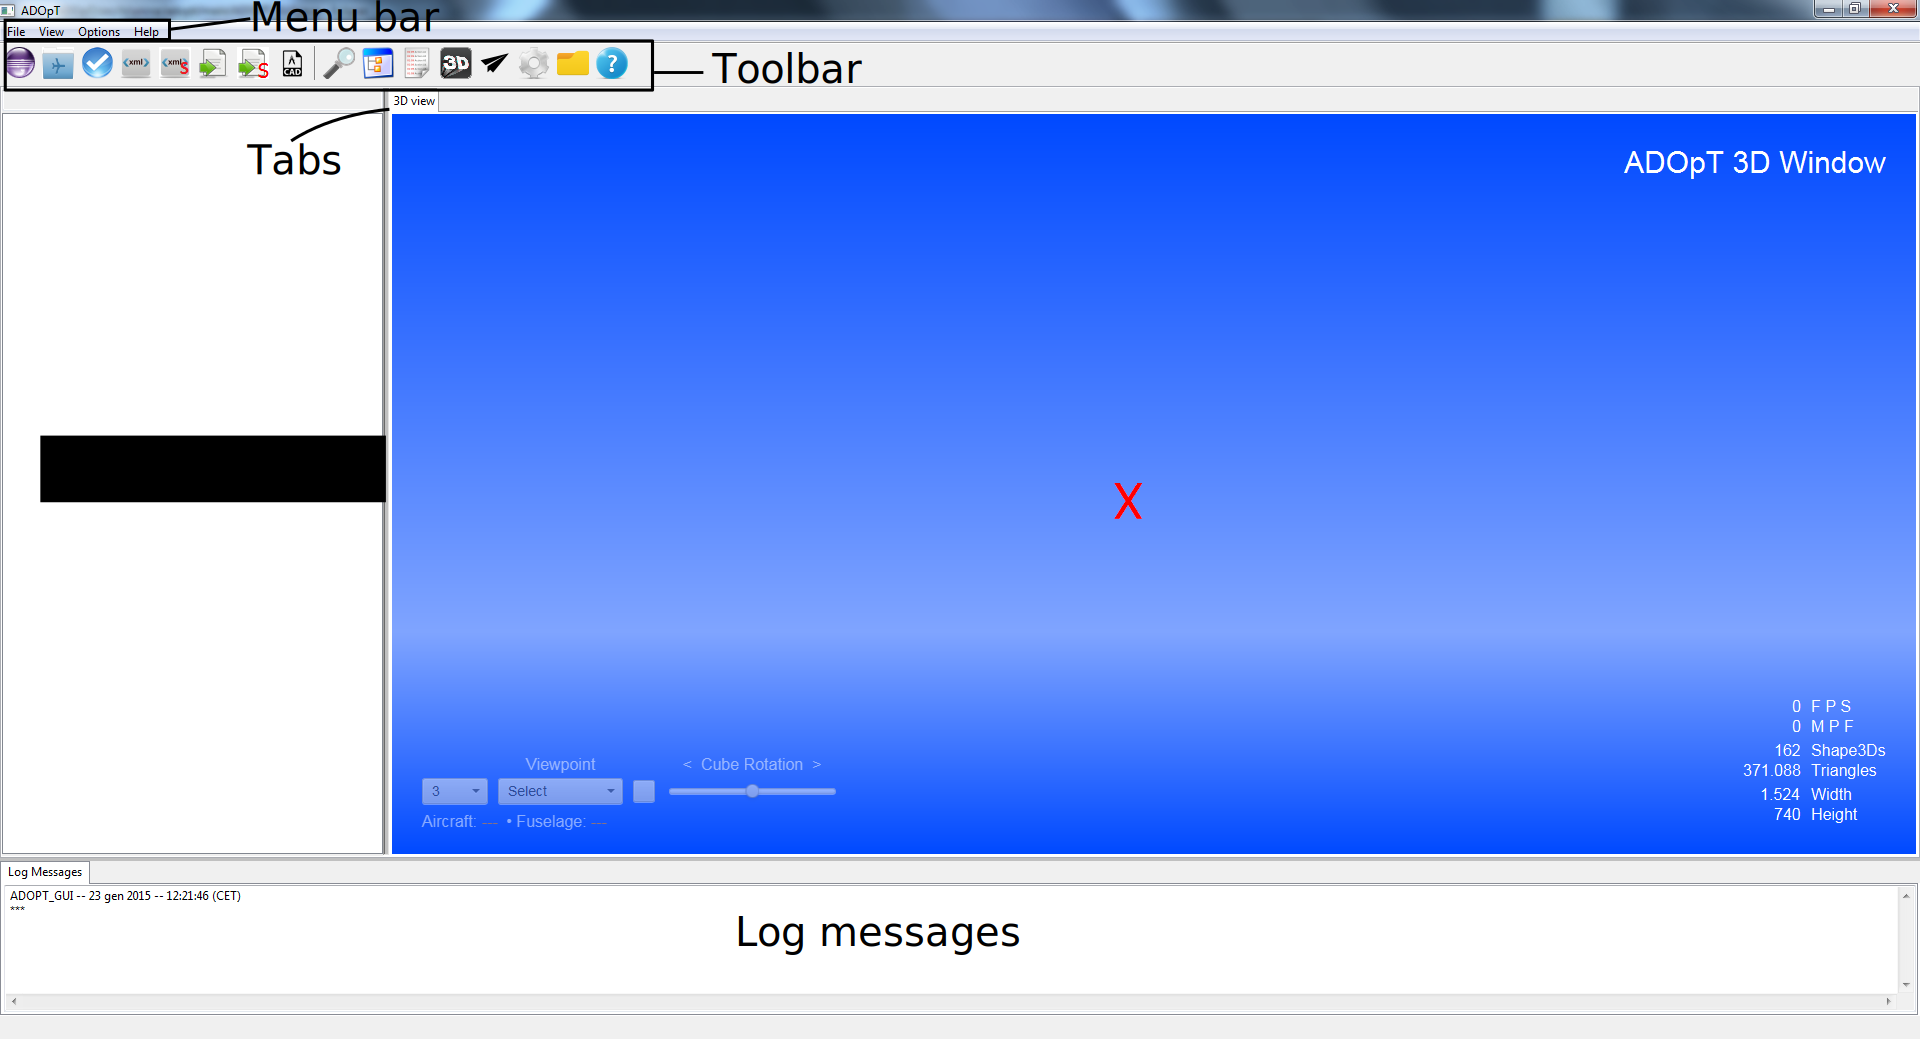
\includegraphics[width=\textwidth]{images/gui/applicationStart}
	\caption{The GUI when the application is started}
	\label{fig:guiStart}
\end{figure}
%
It is composed of several items:
\begin{enumerate}
	\setlength{\itemsep}{\medspacing}
	\item \textbf{Menu bar} (on top), which holds all the available actions divided in sub-categories
	\item \textbf{Toolbar} (below the menu bar), which holds the most important actions needed to interact with the application. The toolbar, as the menu bar, is always visible to the user
	\item \textbf{Project tree} (on the left), a key component of the \gls{acr:GUI} since it provides access to all the components of the aircraft and the analysis results any time during the execution of the application. The project tree appears once an aircraft is created and can be eventually hidden
	\item \textbf{3D view}, which shows the CAD model of the aircraft selected by the user. The CAD model can be updated each time the user wants to check the changes made to the aircraft geometry
	\item \textbf{Log message window}, placed at the bottom, that tells the user the status of pending operations. This window can be hidden
	\item \textbf{Tab folder}, which contains all the windows opened using the project tree; these windows can be closed and reopened any time
\end{enumerate}
%
\subsection{Typical work session}
In developing the application we focused on making the user's typical work session as simple as possible. Few basics steps are required for running an analysis:
%
\begin{enumerate}
	\setlength{\itemsep}{1ex}
	\item Create a new aircraft. This can be done using the corresponding button \big(
\includegraphics[scale=0.6]{images/gui/icons/FolderAirplane_32x32.png}\big) in the toolbar, which instantiates the default aircraft
	\begin{figure}[h]
		\centering
		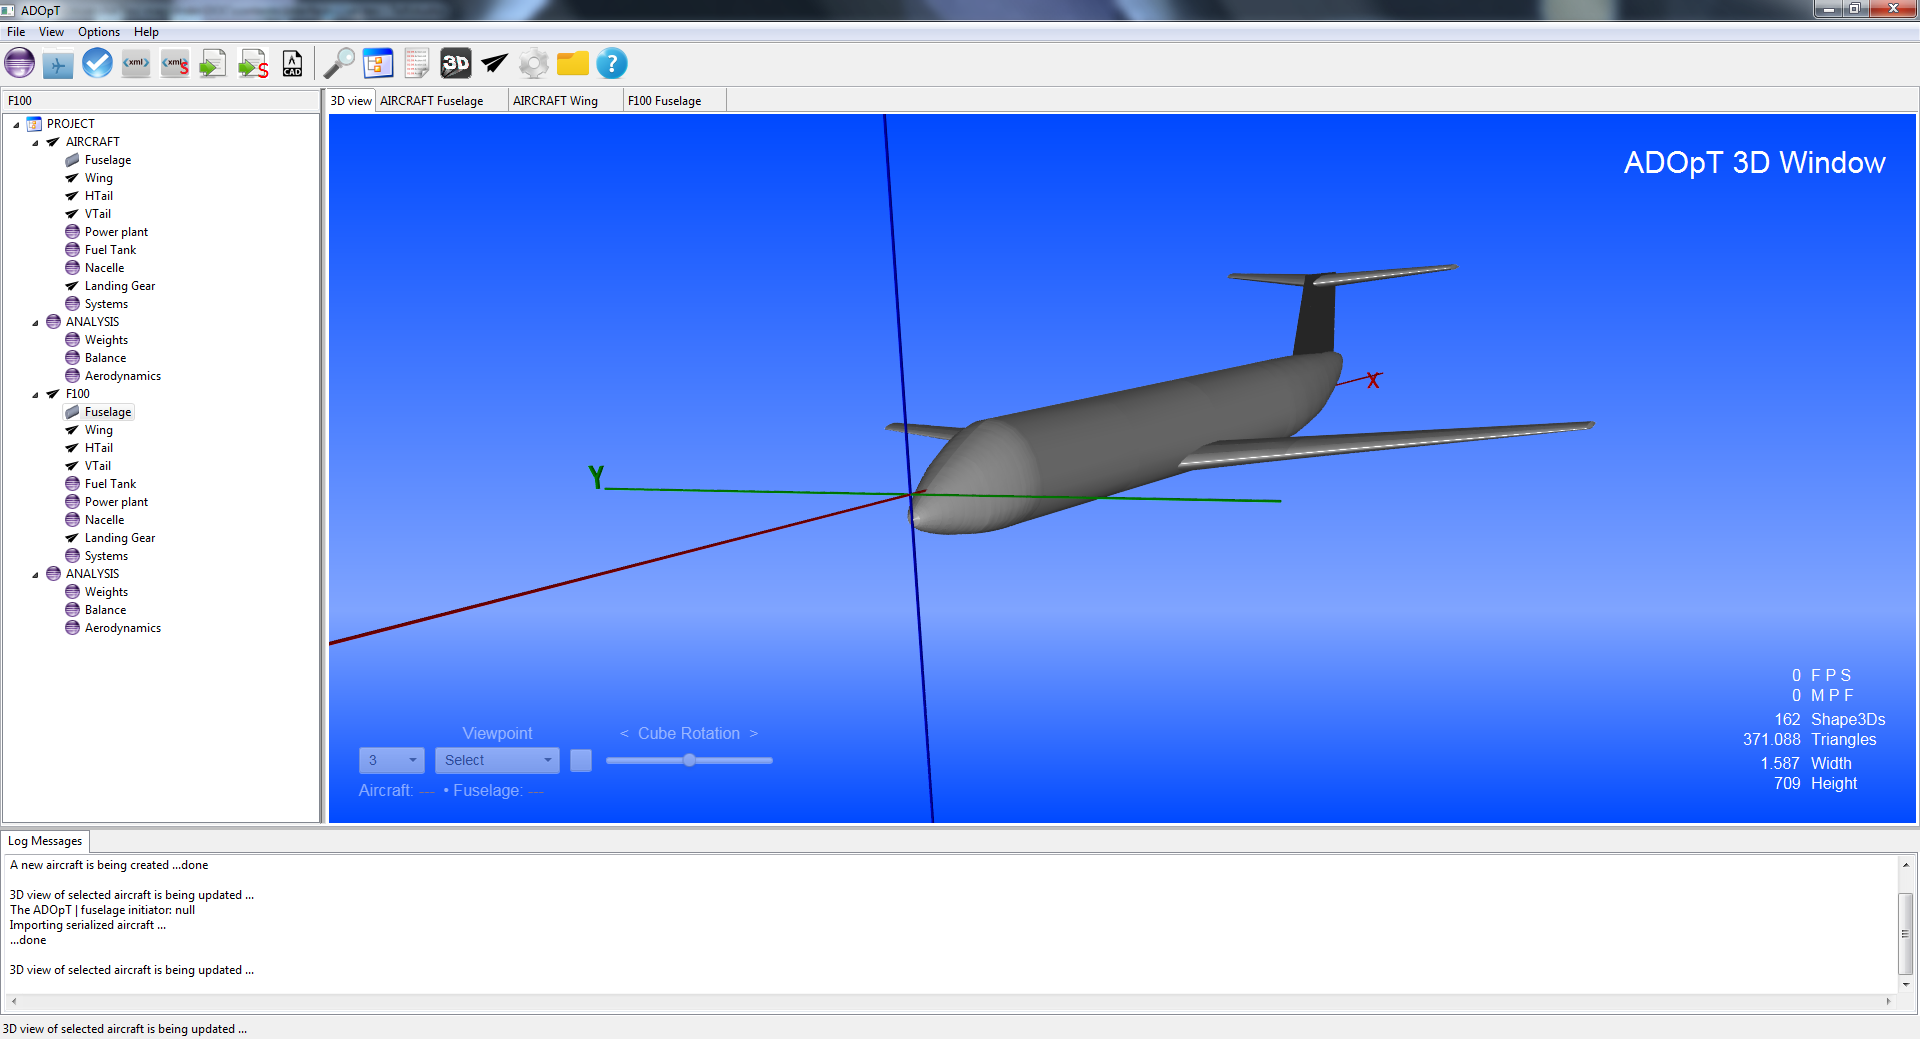
\includegraphics[width=0.93\textwidth,right]{images/gui/createAnotherAircraft}
		\caption{The GUI as it appears when an aircraft is created}
		\label{fig:guiDescription}
	\end{figure}
	
	\item Set the parameters that define the aircraft model using the corresponding window opened using the tree
	\begin{figure}[h]
		\centering
		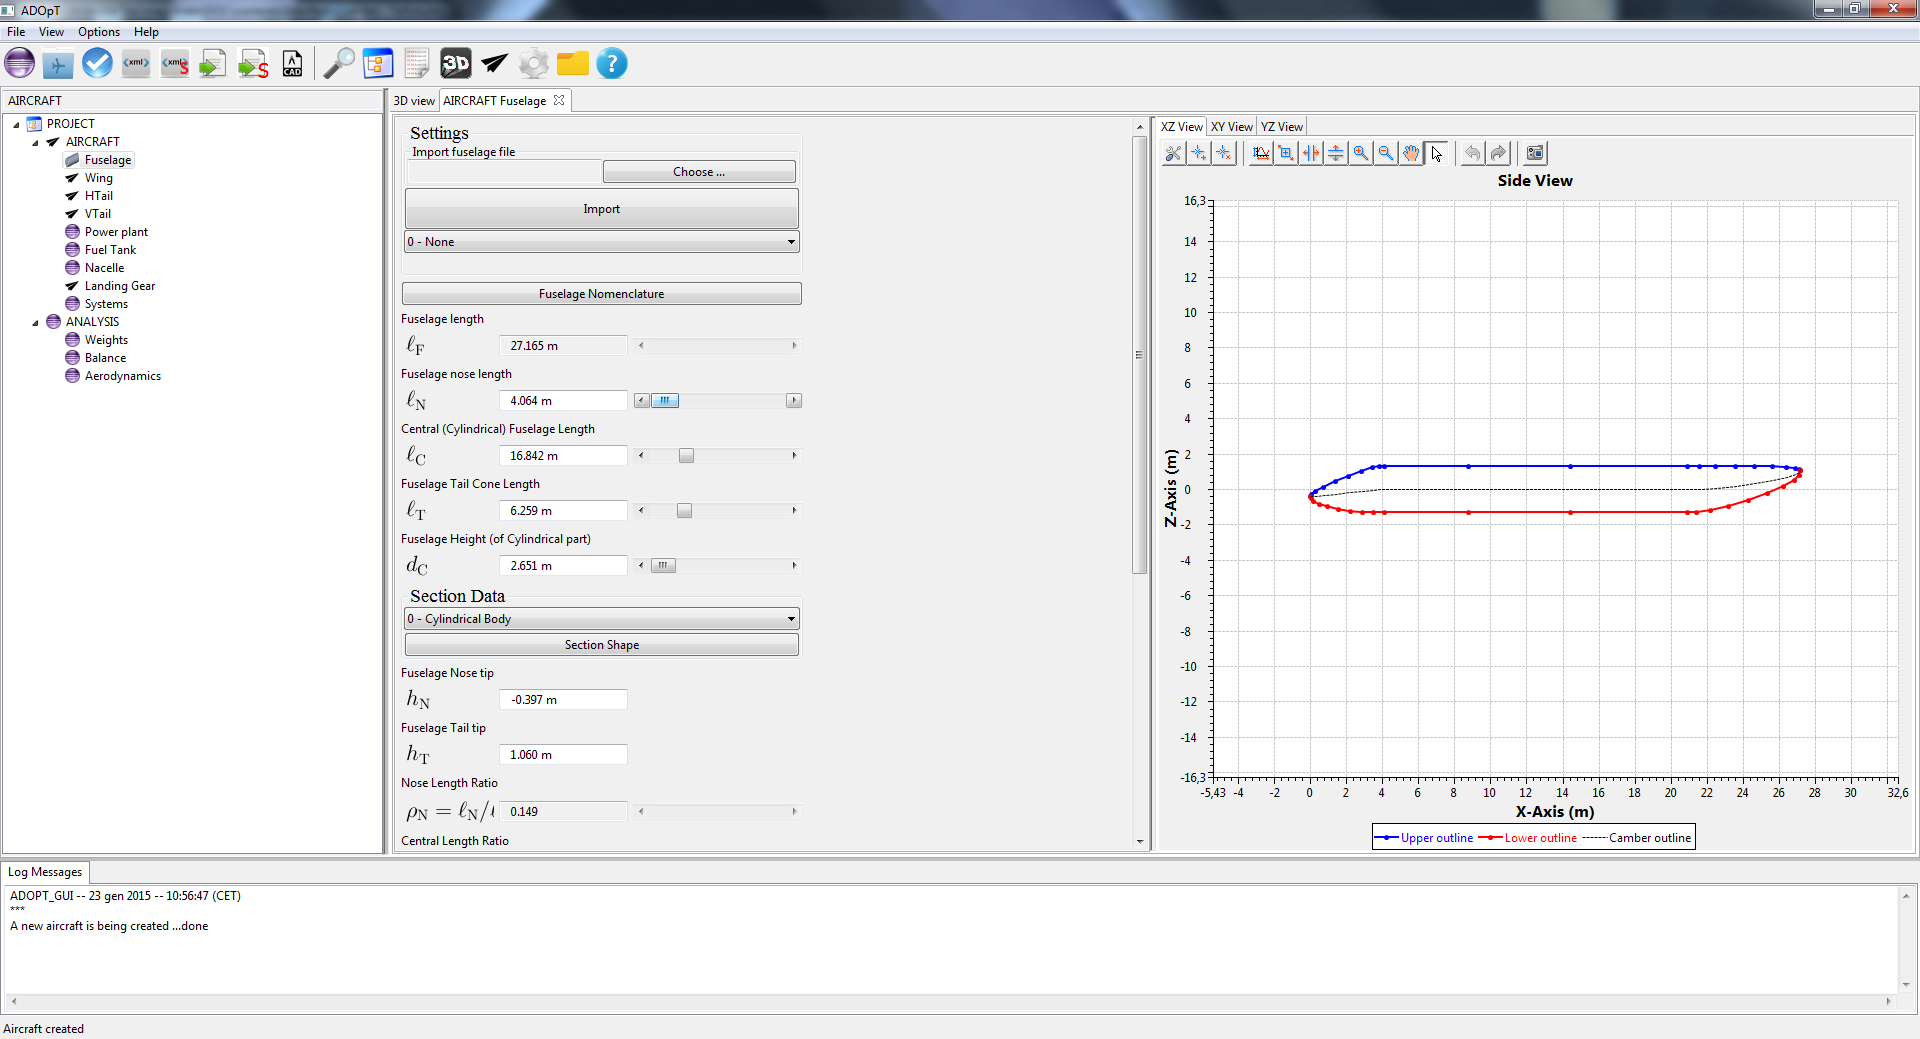
\includegraphics[width=0.93\textwidth,right]{images/gui/changeFusParam}
		\caption{The window for changing the fuselage parameters}
	\end{figure}
	
	\item Explore the 3D model \big(
\includegraphics[scale=1.2]{images/gui/icons/3DView_32x32.png}\big) of the aircraft and eventually change some parameters if there is some error
	\begin{figure}[h]
		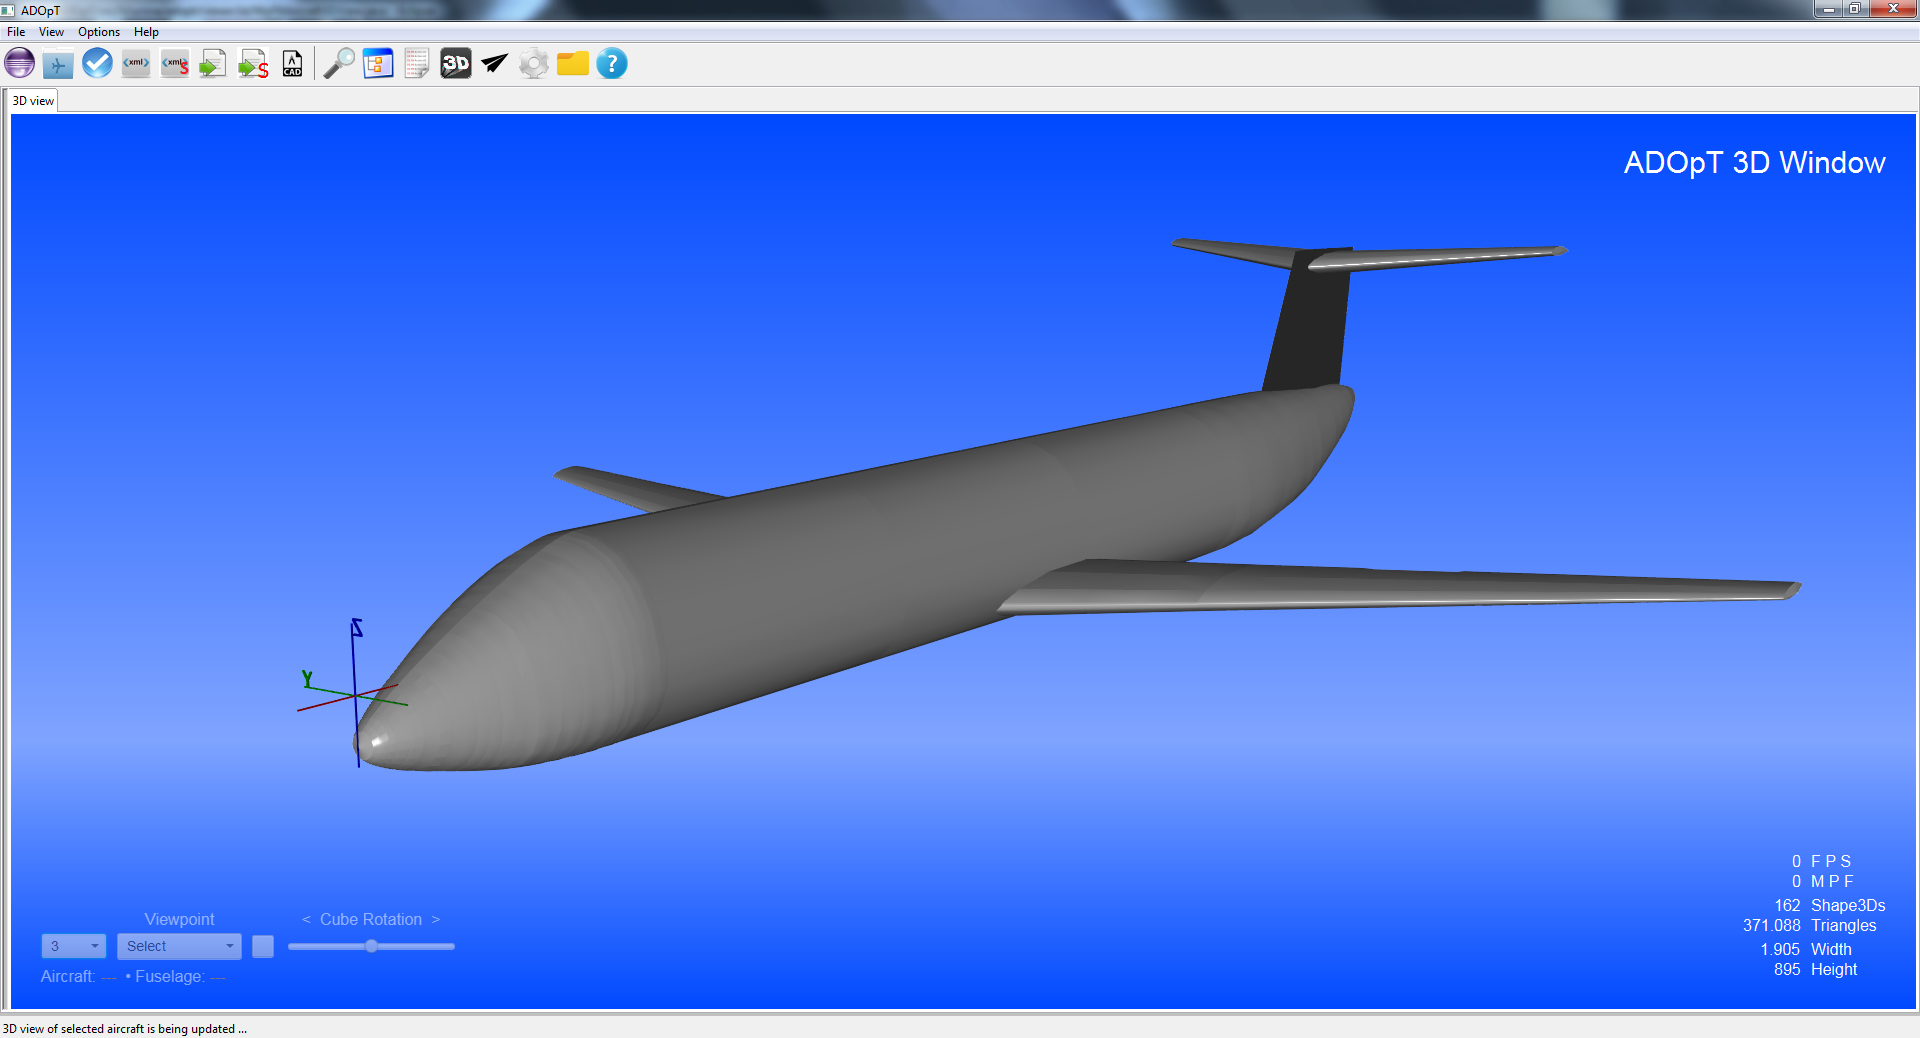
\includegraphics[width=0.93\textwidth,right]{images/gui/explore3D}
		\caption{The aircraft 3D view (log window and project tree hidden)}
	\end{figure}
	
	\item Execute a complete analysis \big(
\includegraphics[scale=0.5]{images/gui/icons/analysis_32x32.png}\big) of the aircraft previously defined

	\item Export the analysis results to an XML and/or an XLS file \big(
\includegraphics[scale=0.4]{images/gui/icons/Export_32x32.png}\big)
	
	\item Eventually export the CAD model of the aircraft \big(
\includegraphics[scale=1.2]{images/gui/icons/cad_32x32.png}\big)
	
	\item Save the current aircraft to an XML file \big(
\includegraphics[scale=0.4]{images/gui/icons/XML_32x32.png}\big)
\end{enumerate}
%
At this point the user could simply change the current configuration until the analysis results are satisfactory. The application can however help the user in finding such a configuration, since it can hold multiple configurations simultaneously, analyse all of them and compare them side by side. To accomplish this task, once the first aircraft has been created, the user should:
%
\begin{enumerate}
	\setlength{\itemsep}{\medspacing}
	\item Import the aicraft previously saved or create an entirely new aircraft
	\item Change the aircraft parameters from the previous step and run a new analysis on it
	\item Study the results and eventually change some of the parameters
	\item Save every configuration and the corresponding results to file
	\item Export both aircraft and the corresponding results to an XLS file
\end{enumerate}
%
Tabs that are related to the same kind of component are distinguished by the aircraft name, put before the component's description, see figure \ref{fig:tabId}.
%
\begin{figure}[H]
	\centering
	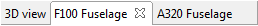
\includegraphics[width=8cm]{images/gui/tabId}
	\caption{Same component tab belonging to different aircraft}
	\label{fig:tabId}
\end{figure}
%
\begin{figure}[H]
	\centering
	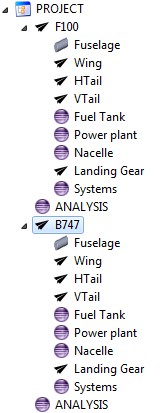
\includegraphics[height=9cm]{images/gui/projectTreeMulti}
	\caption{The project tree holding two different aircraft}
	\label{fig:projectTreeMulti}
\end{figure}
%
There is no limit to the number of aircraft the application can handle; each aircraft is added to the project tree as shown in figure \ref{fig:projectTreeMulti} providing access to the corresponding components and analysis.
%
\subsection{CAD modelling}
The application can also be used as a basic parametric CAD modeler. The capability to change the aircraft parameters using the corresponding controls in the \gls{acr:GUI}, coupled with the 3D view, allows the user to change each component shape and dimension, view the updated CAD model and eventually export it to file once some satisfactory results have been obtained.
%
The CAD model, once saved to a STEP or BRep file, can be imported in CAD suites like FreeCAD, MeshLab, SketchUp, Blender, SolidWorks, or CATIA. The file can also be used to further study the aircraft in a CAE software, such as CD-adapco STAR-CCM+ or ANSYS suite.
%
%-------------------------------OPTIMIZATION------------------------------------
\section{Optimization process}
It has always been the engineer’s dream to have all aspects of analysis done in a relatively short time period so that many different configurations can be examined and the best suitable product can be delivered on time. Although this may still be a dream, actual design turn-around time has become shorter due to the use of mathematical optimization techniques which have been introduced into the design process.\cite{torenbeek2013advanced}

\bigskip
\noindent
According to \cite{howe2000aircraft}, the optimisation of the configuration of the aircraft within the constraints imposed by the specification is an essential feature of the project definition process. Optimisation implies that the proposed design concept not only meets the specification, but does so when a target criterion has been imposed, usually the minimisation of mass or some aspect of costs.
%
The basis of optimisation is a comparison of different design concepts and configuration variations within a given concept to determine the one which best meets the specification. Broadly the process is undertaken at two levels.
%
\begin{itemize}
\item \textbf{Concept/configuration studies} At this level alternative concepts and configurations are investigated to establish the one which would seem best suited to meet the requirements. For example a military combat requirement might possibly be met by aircraft of conventional tail, foreplane or tailless layout. Mostly the configuration of transport aircraft is well established. This phase of the study may be included at the feasibility level.
\item \textbf{Parametric studies within a given configuration} At this level the dominant parameters are varied to ascertain the best combination of them. These parameters include such items as wing geometry determined by aspect ratio, sweep, taper and thickness as well as variations in fuselage layout, powerplant installation and so on. The benefits of selecting near optimum values of certain parameters are "traded-off" against the implied penalties
imposed upon other parameters. The parametric studies may be commenced during feasibility investigations and certainly form a major part of the project definition phase. The two fundamental design characteristics which drive the parametric studies are:
\begin{itemize}
\item Wing loading, that is wing area as a function of take-off mass or weight
\item Thrust or power loading, defined as the ratio of the basic powerplant to the aircraft mass or weight
\end{itemize}
\end{itemize}
%
It is, precisely, the latter type of optimization which will be the main feature to implement inside \gls{JPAD} in the near future. As all analysis modules inside the \lstinline[language=Java]!JPADCore! package will be completed and tested, the final purpose of the code will be to allow users to define a certain numbers of macroscopical geometrical parameters, along with a given objective function, and to receive as output the best set of the previous parameters which suits the wanted objective.















